\subsection{Simulaciones}
\bigskip
\subsubsection{Polarización}

\begin{figure}[H]
\centering
\centerline{
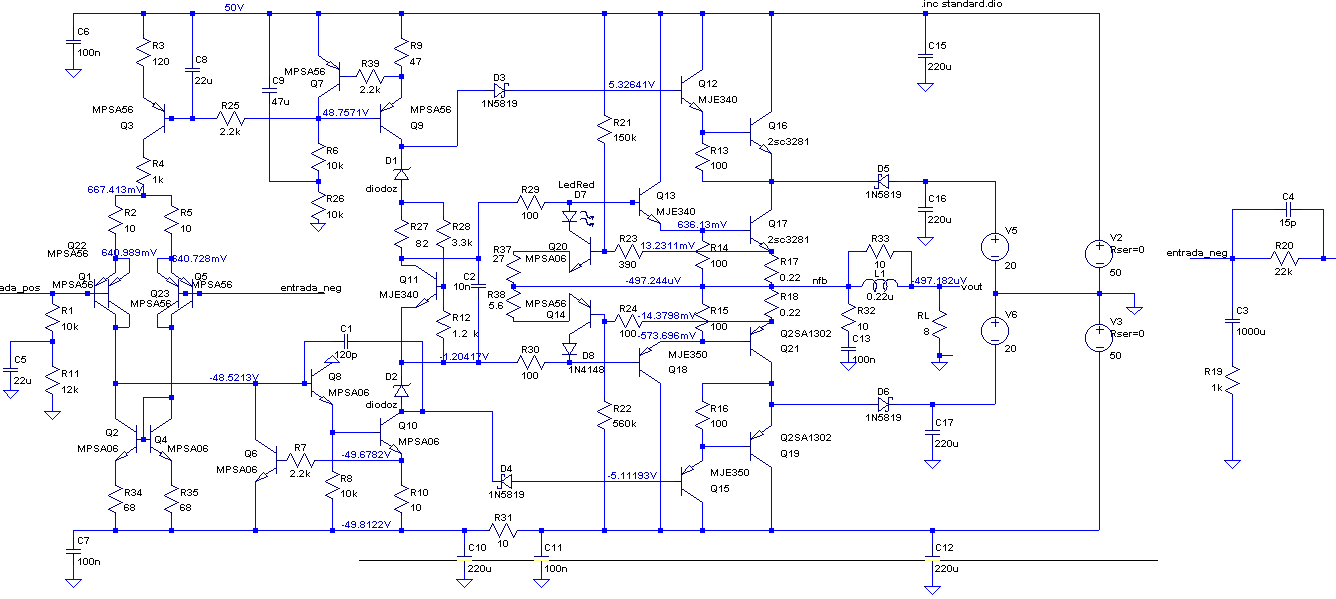
\includegraphics[width=\textwidth]{img/polarizacion.png}}
\caption{Tensiones de polarización.}
\label{polarizacion_sim} 
\end{figure}
\medskip
\subsubsection{Respuesta en Frecuencia}

Se realizó un barrido en frecuencias de la ganancia del circuito a lazo cerrado para poder observar el ancho de banda del mismo. Como resultado se obtuvo una ganancia de 27.19dB y y se mantiene en el mismo con un error de $\pm$0.1dB entre 5Hz y 66.55kHz.
Estos resultados se pueden observar en la Figura~\ref{resp_frec}, por lo tanto el diseño cumple el requerimiento de banda plana en las frecuencias utilizadas. 

\begin{figure}[H]
\centering
\centerline{
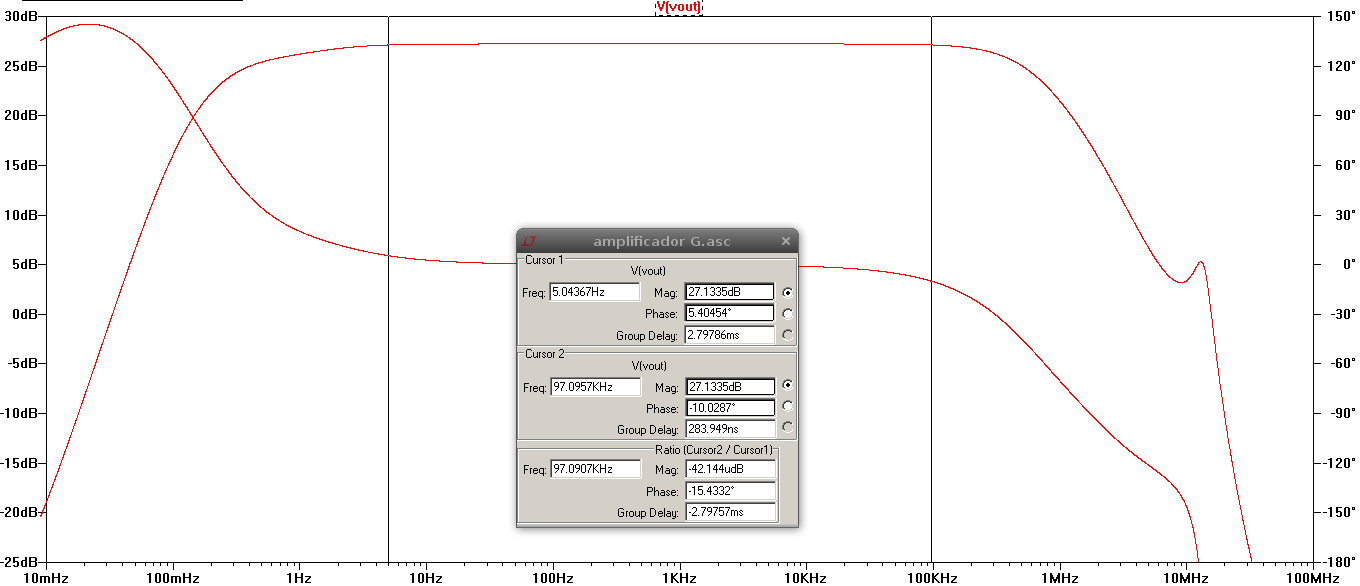
\includegraphics[width=\textwidth]{img/ancho_de_banda.png}}
\caption{Respuesta en frecuencia.}
\label{resp_frec} 
\end{figure}

\bigskip
\subsubsection{Slew Rate}

Para esta simulación se utilizo el circuito de la Figura~\ref{cir_simul_slew_rate}, en el cual la entrada al amplificador es una señal escalón. Se simuló y se tomaron las tensiones en dos puntos, luego se aproxima el slew rate como la pendiente entre estos puntos. Como se ve en la Figura~\ref{simul_slew_rate} con los puntos elegidos se obtuvo un slew rate de $37~ \frac{\volt}{\usec}$.

\begin{figure}[H]
\centering
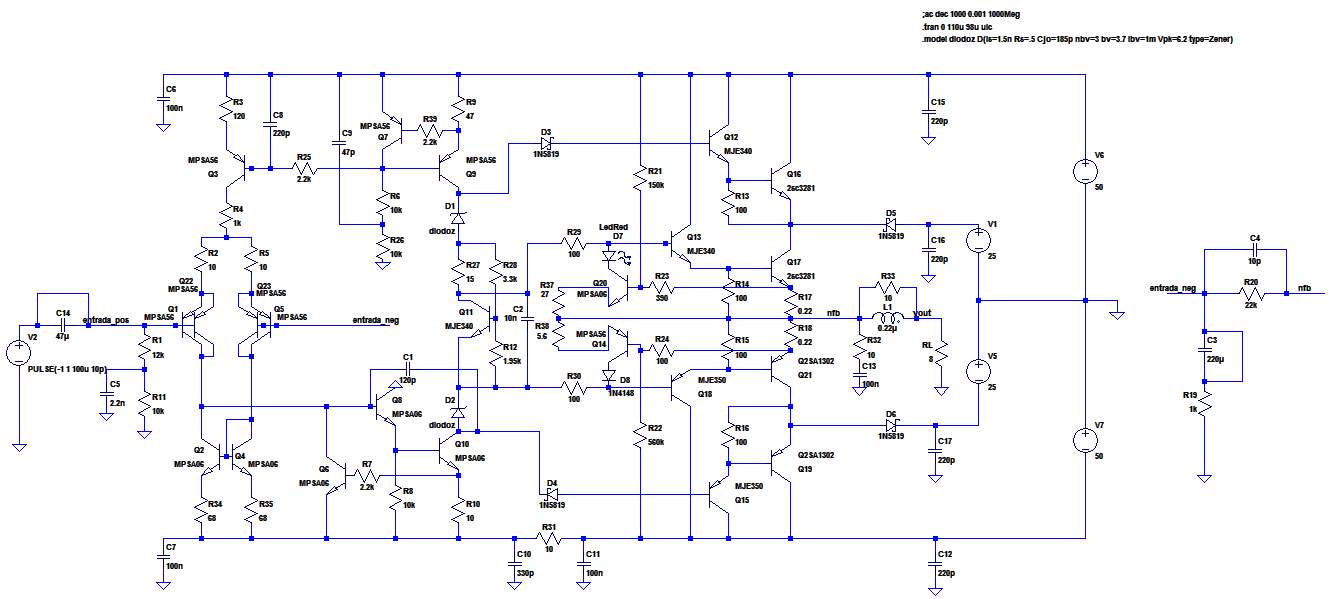
\includegraphics[width=1\textwidth]{img/slew_rate_cir.png}
\caption{Circuito utilizado para obtener slew rate.}
\label{cir_simul_slew_rate}
\end{figure}

\begin{figure}[H]
\centering
\centerline{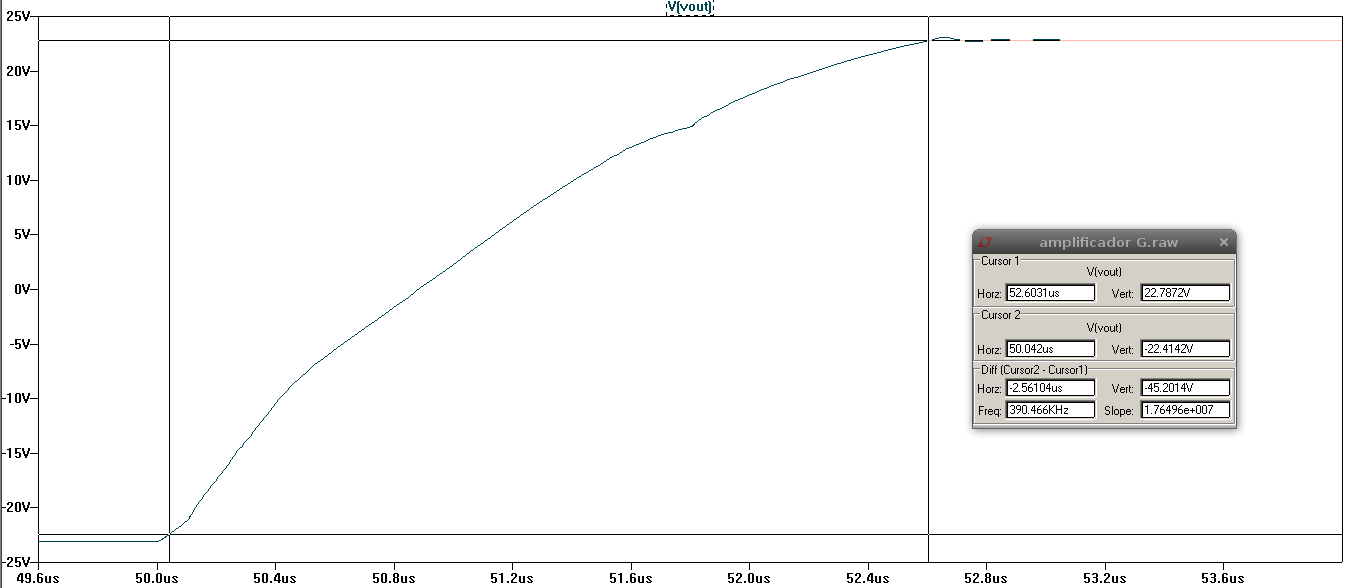
\includegraphics[width=1\textwidth]{img/slew_rate.png}}
\caption{Simulación del slew rate.}
\label{simul_slew_rate}
\end{figure}

\medskip
\subsubsection{Estabilidad}

Para obtener el margen de ganancia y fase del circuito se simuló la respuesta en frecuencia de la ganancia a lazo abierto(T), para esto se modificó la topologia del circuito como se ve en la Figura~\ref{cir_simul_estab}. Para obtener el margen de ganancia se determino la ganancia con un angulo de -180º, dando un margen de 3.9dB. Por otro lado, el margen de fase resulto de 72º,siendo la diferencia entre la fase a 0dB y -180º.
Los resultados de la simulación se observan en la Figura~\ref{simul_estab}.

\begin{figure}[H]
\centering
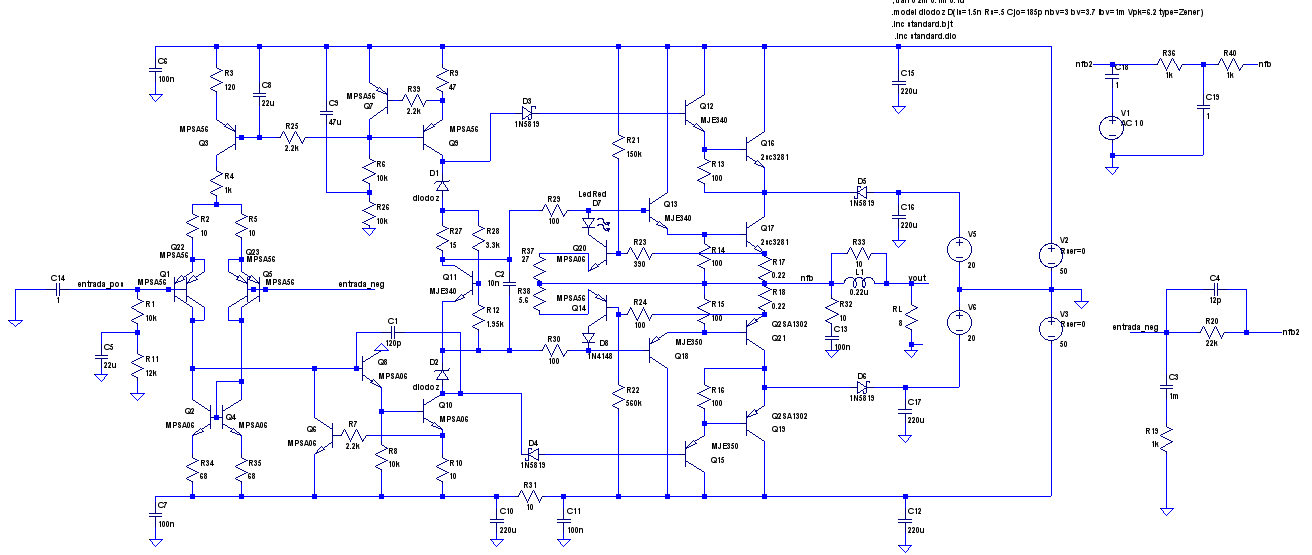
\includegraphics[width=1\textwidth]{img/margen_fase_ganancia_cir.png}
\caption{Circuito utilizado en análisis de estabilidad.}
\label{cir_simul_estab}
\end{figure}


\begin{figure}[H]
\centering
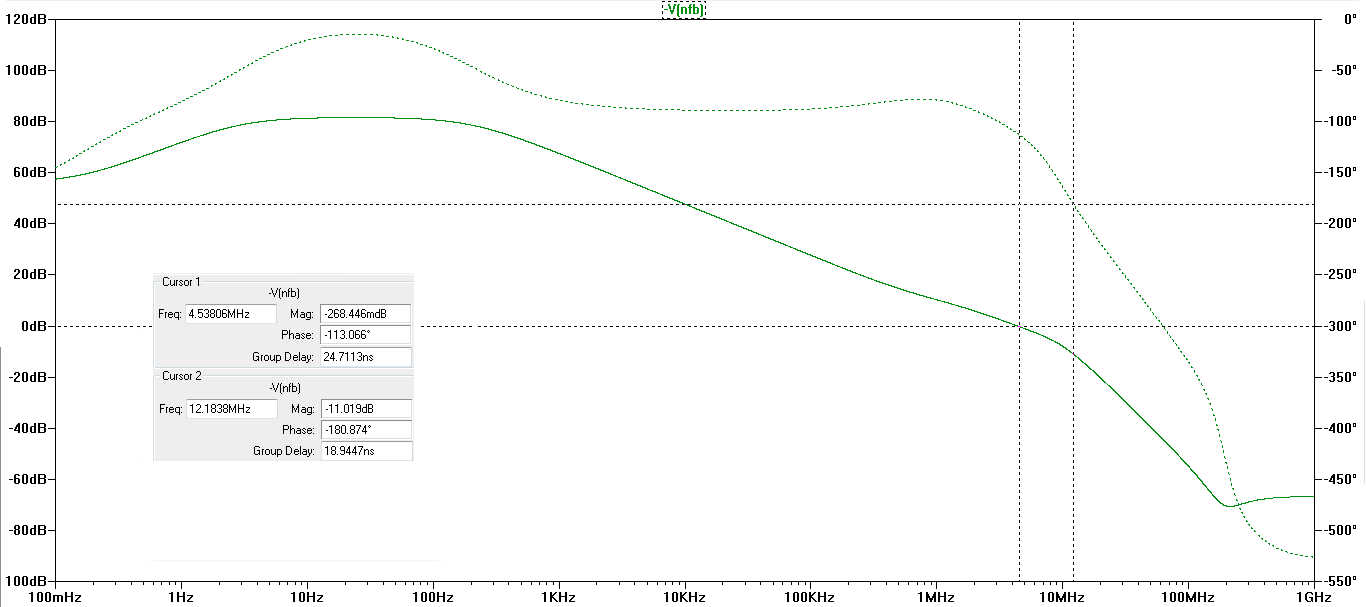
\includegraphics[width=1\textwidth]{img/margen_fase_ganancia.png}
\caption{Respuesta en frecuencia de T.}
\label{simul_estab}
\end{figure}

\medskip
\subsubsection{Eficiencia}

\begin{figure}[H]
\centering
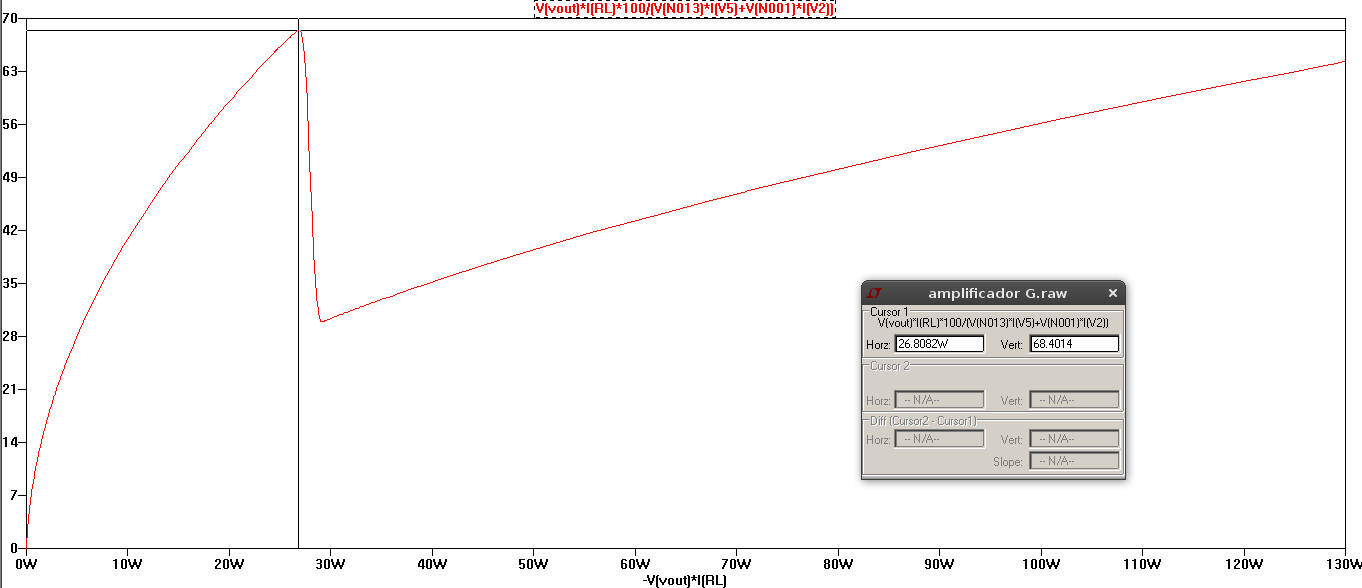
\includegraphics[width=1\textwidth]{img/eficiencia.png}
\caption{Eficiencia del amplificador en función a la potencia disipada en la carga.}
\label{simul_efi}
\end{figure}

\subsubsection{Impedancia de entrada}

Para simular la impedancia de entrada simplemente se puso una fuente de señal a la entrada y se dividió por la corriente que pasaba por ella. Mostramos ahora los resultados de esa simulación.

\begin{figure}[H]
\centering
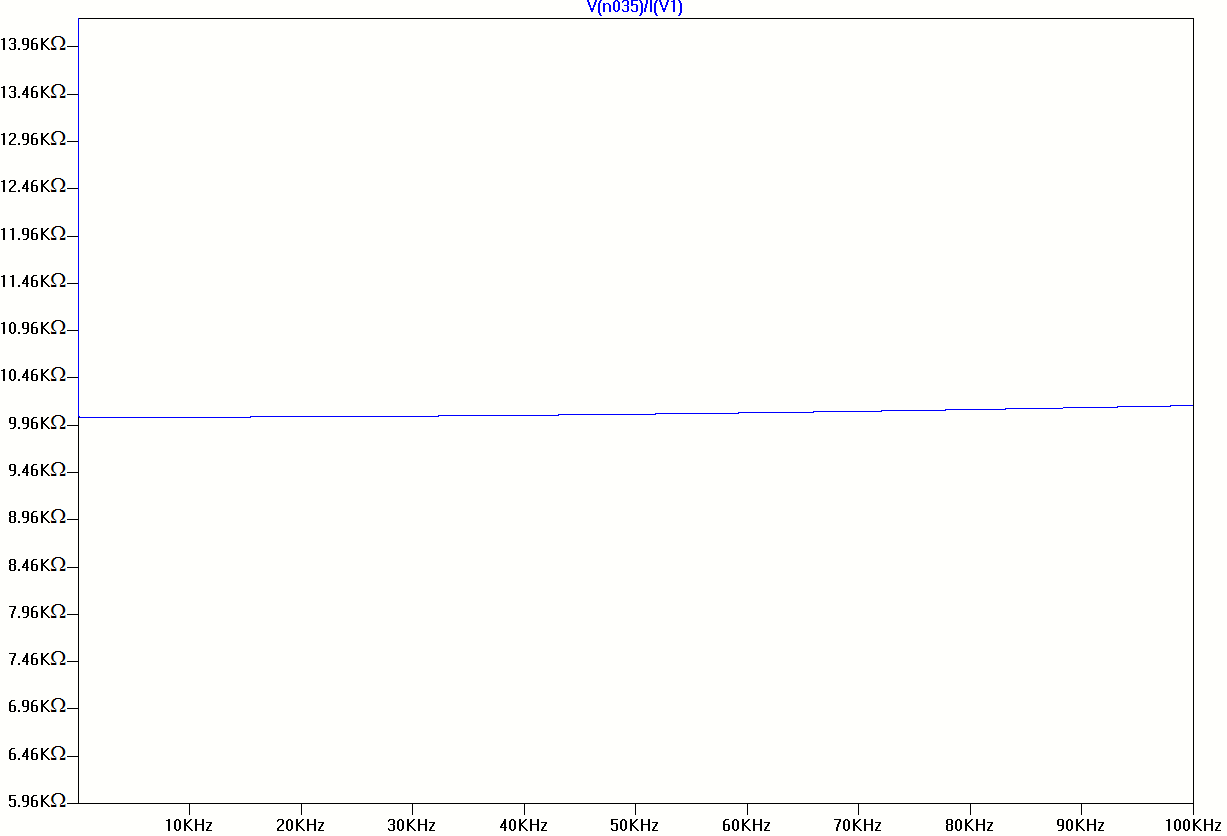
\includegraphics[width=1\textwidth]{img/Rin.png}
\caption{Resistencia de entrada en función de la frecuencia.}
\label{Rin_sim}
\end{figure}

\subsubsection{Impedancia de salida}

La impedacia de salida se la simuló de dos formas. Una aplicando Thévenin y pasivando la entrada, poniendo una fuente de señal a la salida desacoplada por un capacitor, como se ve en la figura.

\begin{figure}[H]
\centering
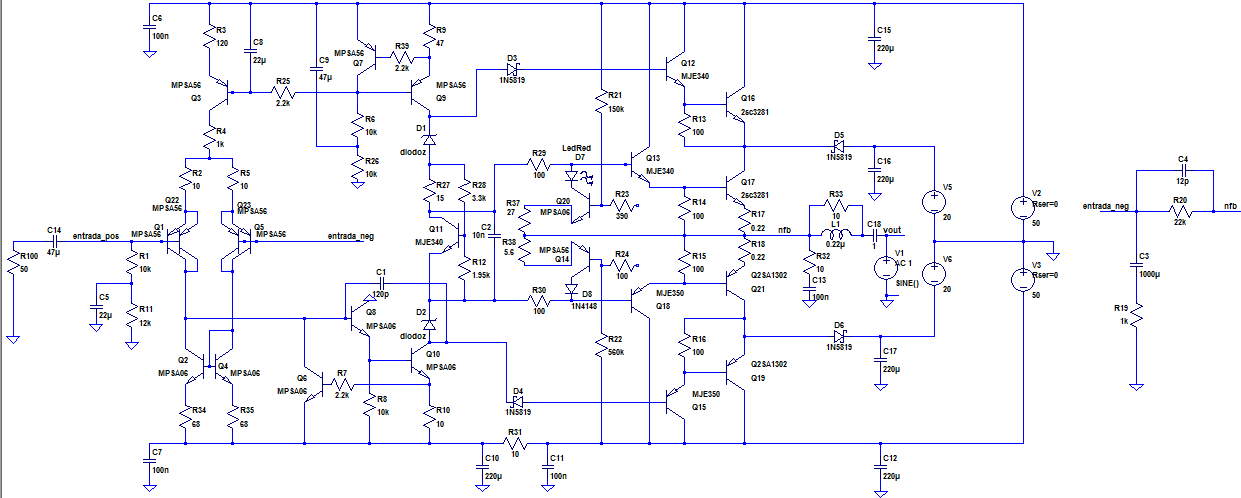
\includegraphics[width=1\textwidth]{img/Rout_circ_1.png}
\caption{Circuito para la simulación de la impedancia de salida.}
\label{Rout_sim_circ}
\end{figure}

Luego se dividió la corriente que pasaba por ella por la tensión y tenemos la impedancia vista por la entrada en función de la frecuencia.

\begin{figure}[H]
\centering
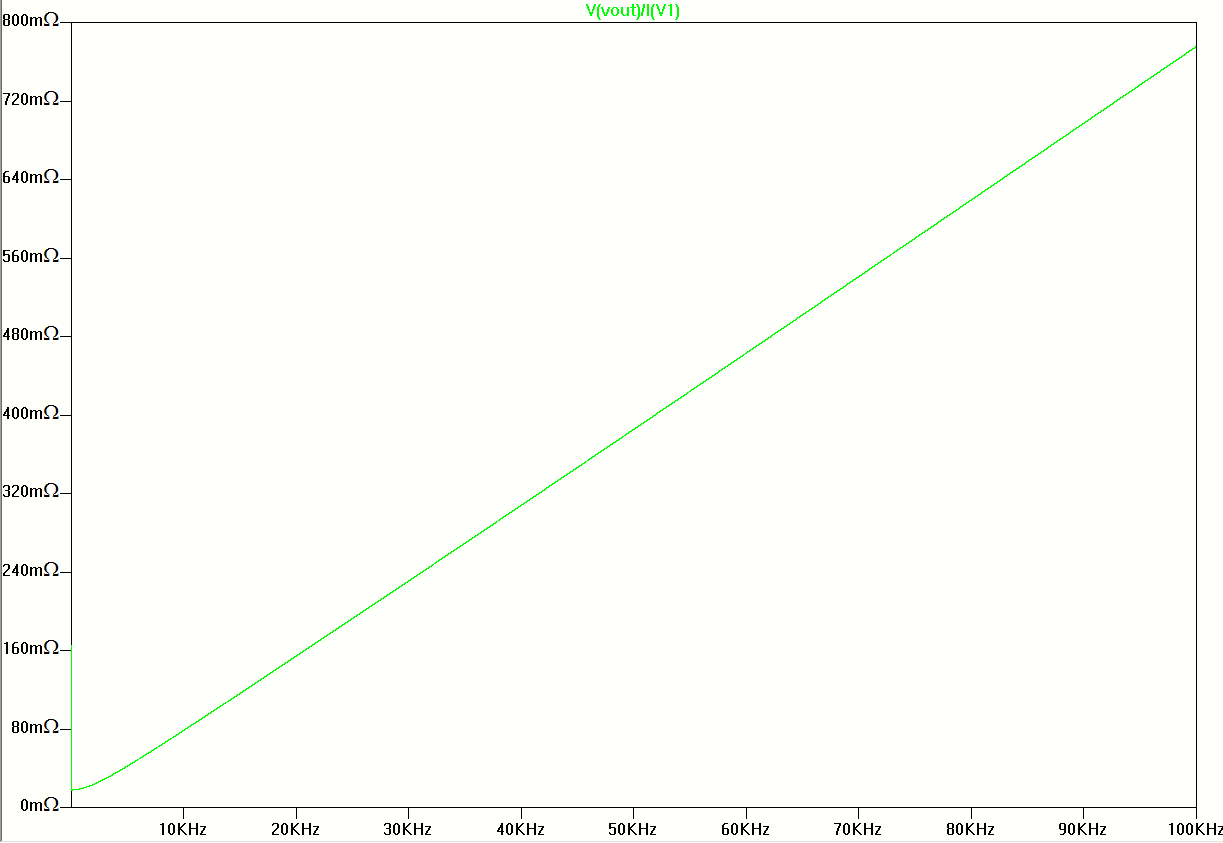
\includegraphics[width=1\textwidth]{img/Rout_1.png}
\caption{Simulación de la impedancia de salida.}
\label{Rout_sim}
\end{figure}

La otra simulación que se hizo fue la de la misma medición. Poniendo carga infinita y de $8\ohm$, luego aproximando con $R_{out}=8\ohm(\frac{V_{\inf}}{V_{8\ohm}}-1)$.

\begin{figure}[H]
\centering
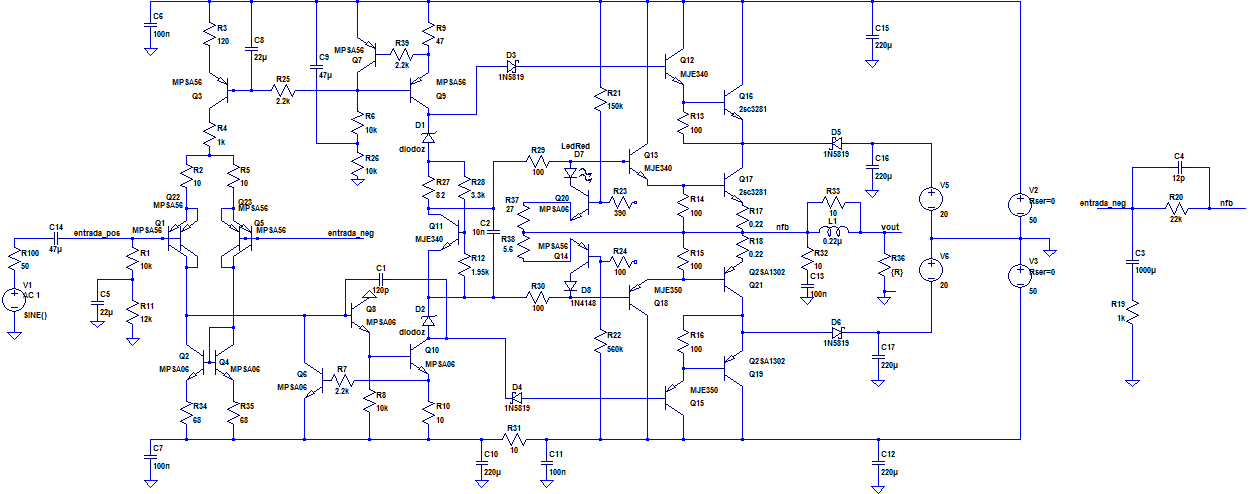
\includegraphics[width=1\textwidth]{img/Rout_circ_2.png}
\caption{Circuito para la medición de la impedancia de salida.}
\label{Rout_med_circ}
\end{figure}

El resultado obtenido a $1kHz$ que fue la frecuencia a la que se lo midió, se puede ver en la figura. El resultado de la aproximación es de $18m\ohm$.

\begin{figure}[H]
\centering
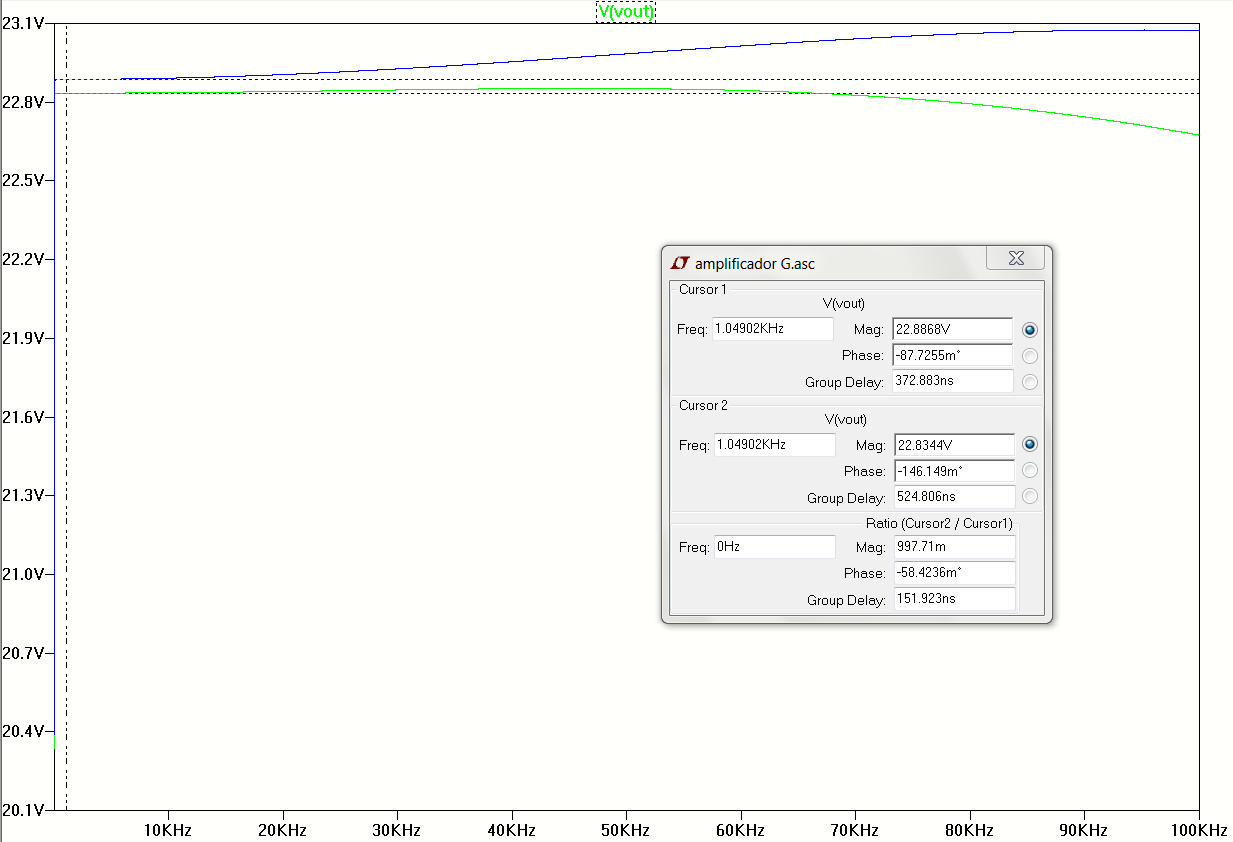
\includegraphics[width=1\textwidth]{img/Rout_2.png}
\caption{Simulación de la medición de la impedancia de salida.}
\label{Rout_med}
\end{figure}

\subsubsection{Distorsión}

Se simuló el circuito para cada caso en el que se midió distorsión, dando los siguientes resultados.

\begin{itemize}
\item A $0.3V_{rms}$, $1kHz$, sin carga: THD=$0.011222\%$
\item A $0.3V_{rms}$, $7kHz$, sin carga: THD=$0.014968\%$
\item A $0.3V_{rms}$, $1kHz$, con carga: THD=$0.002572\%$
\item A $0.3V_{rms}$, $7kHz$, con carga: THD=$0.015194\%$
\item A $1V_{rms}$, $1kHz$, sin carga: THD=$0.001564\%$
\item A $1V_{rms}$, $7kHz$, sin carga: THD=$0.015398\%$
\item A $1V_{rms}$, $1kHz$, con carga: THD=$0.008341\%$
\item A $1V_{rms}$, $7kHz$, con carga: THD=$0.037159\%$
\end{itemize}